\begin{center}
  \section*{Homework 03 - 2.5}
  Due Feb 27 \\
  Uzair Hamed Mohammed
\end{center}

% 6, 8, 14, 20, 24

\begin{enumerate}
  \item[6.] Three points, \(X_1, X_2,\) and \(X_3\), are chosen at random in the
    interval $(0, a)$. A second set of three points, $Y_1$, $Y_2$, and $Y_3$,
    are chosen at random in the interval $(0, b)$. Let $A$ be the event
    that $X_2$ is between $X_1$ and $X_3$. Let $B$ be the event that
    $Y_1 < Y_2 <
    Y_3$. Find $P(A \cap B)$.

    \underline{Sol}: We can expect the second random variable \(Y_2\)
    to be in the middle. Given this information, as events A and B
    are independent, we get:
    \[
      P(A \cap B) = P(A) P(B) = \boxed{\frac{1}{9}}
    \]

  \item[8.] Suppose that events A, B, and C are independent.
    \begin{enumerate}
      \item Use a Venn diagram to find an expression for \(P(A \cup B
        \cup C)\) that does not make use of a complement.

        \underline{Sol}:
        \begin{center}
          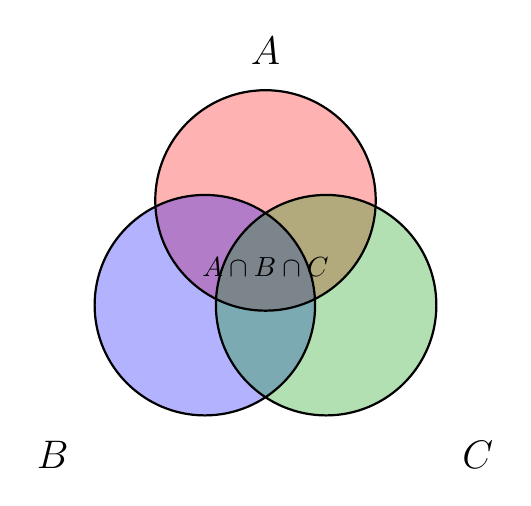
\begin{tikzpicture}[thick, scale=0.7]
            % 1. Define the centers of the circles
            \coordinate (A) at (0,1.2);
            \coordinate (B) at (-1.1, -0.7);
            \coordinate (C) at (1.1, -0.7);

            % 2. Fill the circles with transparency (multiply mode
            % makes intersections darker)
            \begin{scope}[fill opacity=0.3]
              \fill[red] (A) circle (2cm);
              \fill[blue] (B) circle (2cm);
              \fill[green!60!black] (C) circle (2cm);
            \end{scope}

            % 3. Draw the outlines
            \draw (A) circle (2cm) node[above=1.6cm] {\Large $A$};
            \draw (B) circle (2cm) node[below left=1.6cm] {\Large $B$};
            \draw (C) circle (2cm) node[below right=1.6cm] {\Large $C$};

            % 4. Add the center intersection label
            \node at (0,0) {$A \cap B \cap C$};
          \end{tikzpicture}
        \end{center}
        \[
          \begin{aligned}
            P(A \cup B \cup C) = P(A) + P(B) + P(C) - [P(A)P(B) + \\
            P(A)P(C) + P(B)P(C)] + P(A)P(B)P(C)
          \end{aligned}
        \]
      \item Find an expression for \(P(A \cup B \cup C)\) that does
        make use of a complement.

        \underline{Sol}:
        \[
          \begin{aligned}
            1 - P((A \cup B \cup C)^C) &= 1 - P(A^C \cap B^C \cap C^C) \\
            &= 1 - P(A^C) P(B^C) P(C^C)
          \end{aligned}
        \]
    \end{enumerate}

  \item[14.] In a roll of a pair of fair dice (one red and one
    green), let A be the event the red die shows a 3, 4, or 5; let B
    be the event the green die shows a 1 or a 2; and let C be the
    event the dice total is 7. Show that A, B, and C are independent.

    \underline{Sol}: If we consider the probabilities of different
    events we will see the equities needed for independence clearly:

    \begin{itemize}
      \item \(P(A) = \frac{18}{36} = \frac{1}{2}\)
      \item \(P(B) = \frac{12}{36} = \frac{1}{3}\)
      \item \(P(C) = \frac{6}{36} = \frac{1}{6}\)
      \item \(P(A \cap B) = \frac{6}{36} = \frac{1}{6} = P(A) P(B)\)
      \item \(P(A \cap C) = \frac{3}{36} = \frac{1}{12} = P(A) P(C)\)
      \item \(P(B \cap C) = \frac{2}{36} = \frac{1}{18} = P(B) P(C)\)
      \item \(P(A \cap B \cap C) = \frac{1}{36} = P(A) P(B) P(C)\)
    \end{itemize}

  \item[20.] Players A, B, and C toss a fair coin in order. The first
    to throw a head wins. What are their respective chances of winning?

    \underline{Sol}: For person A,
    \[
      \begin{aligned}
        P(A) &= \frac{1}{2} + (\frac{1}{2})^3 \frac{1}{2} +
        (\frac{1}{2}) + \dots \\
        &= \frac{1}{2} \sum_{k = 0}^{\infty} (\frac{1}{2})^{3k} \\
        &= \frac{1}{2} (\frac{1}{1 - \frac{1}{8}}) \\
        &= \boxed{\frac{4}{7}}
      \end{aligned}
    \]

    For person B,
    \[
      \begin{aligned}
        P(B) &= \frac{1}{2} (\frac{1}{2}) + \frac{1}{2}
        (\frac{1}{2})^3 \frac{1}{2} + \frac{1}{2} (\frac{1}{2})^6
        \frac{1}{2} + \dots \\
        &= \frac{1}{4} \sum_{k = 0}^{\infty} (\frac{1}{2})^{3k} \\
        &= \frac{1}{4} (\frac{1}{1 - \frac{1}{8}}) \\
        &= \boxed{\frac{2}{7}}
      \end{aligned}
    \]

    For person C,
    \[
      \begin{aligned}
        P(C) &= (\frac{1}{2})^2 (\frac{1}{2}) + (\frac{1}{2})^2
        (\frac{1}{2})^3 \frac{1}{2} + (\frac{1}{2})^2 (\frac{1}{2})^6
        \frac{1}{2} + \dots \\
        &= \frac{1}{8} \sum_{k=0}^{\infty} (\frac{1}{2})^{3k} \\
        &= \frac{1}{8} (\frac{1}{1 - \frac{1}{8}}) \\
        &= \boxed{\frac{1}{7}}
      \end{aligned}
    \]

  \item[24.] Each of m urns contains three red chips and four white
    chips. A total of r samples with replacement are taken from each
    urn. What is the probability that at least one red chip is drawn
    from at least one urn?

    \underline{Sol}: Since each urn has the same distribution of red
    and white chips,

    \begin{itemize}
      \item \(P(\textrm{red chip}) = \frac{3}{7}\)
      \item \(P(\textrm{no red chip from r draws in a single urn}) = (1 - p)^r\)
      \item \(P(\textrm{no red chip from any of r draws from each of
        the m urns}) = (1-p)^{rm}\)
      \item \(P(\textrm{at least one red chip}) = \boxed{1-(1-p)^{rm}}\)
    \end{itemize}

\end{enumerate}
